\usepackage{xcolor}
\usepackage{afterpage}
\usepackage{pifont,mdframed}
\usepackage[bottom]{footmisc}
\usepackage{minted}

\createsection{\Grader}{Grader di prova}
\newcommand{\inputfile}{\texttt{stdin}}
\newcommand{\outputfile}{\texttt{stdout}}
\makeatletter
\renewcommand{\this@inputfilename}{\texttt{stdin}}
\renewcommand{\this@outputfilename}{\texttt{stdout}}
\renewcommand{\this@syllabuslevel}{5}
\renewcommand{\this@custdifficulty}{3}
\makeatother

% % % % % % % % % % % % % % % % % % % % % % % % % % % % % % % % % % % % % % % % % % %
% % % % % % % % % % % % % % % % % % % % % % % % % % % % % % % % % % % % % % % % % % %
Ultimamente Andrea si sta dedicando alla scrittura, e ha quasi finito di scrivere il suo capolavoro:
\textbf{\textit{Sussone Fundamenta Prima}}, un libro che raccoglie le tecniche base della programmazione
che permettono al lettore di aprire la mente e di "\textit{Sussarsi}" \textit{cit. Sussone Fundamenta Prima}.

Per rendere il tomo più interessante, decide di numerare le pagine secondo un ordine particolare.

\begin{figure}[h]
    \centering
    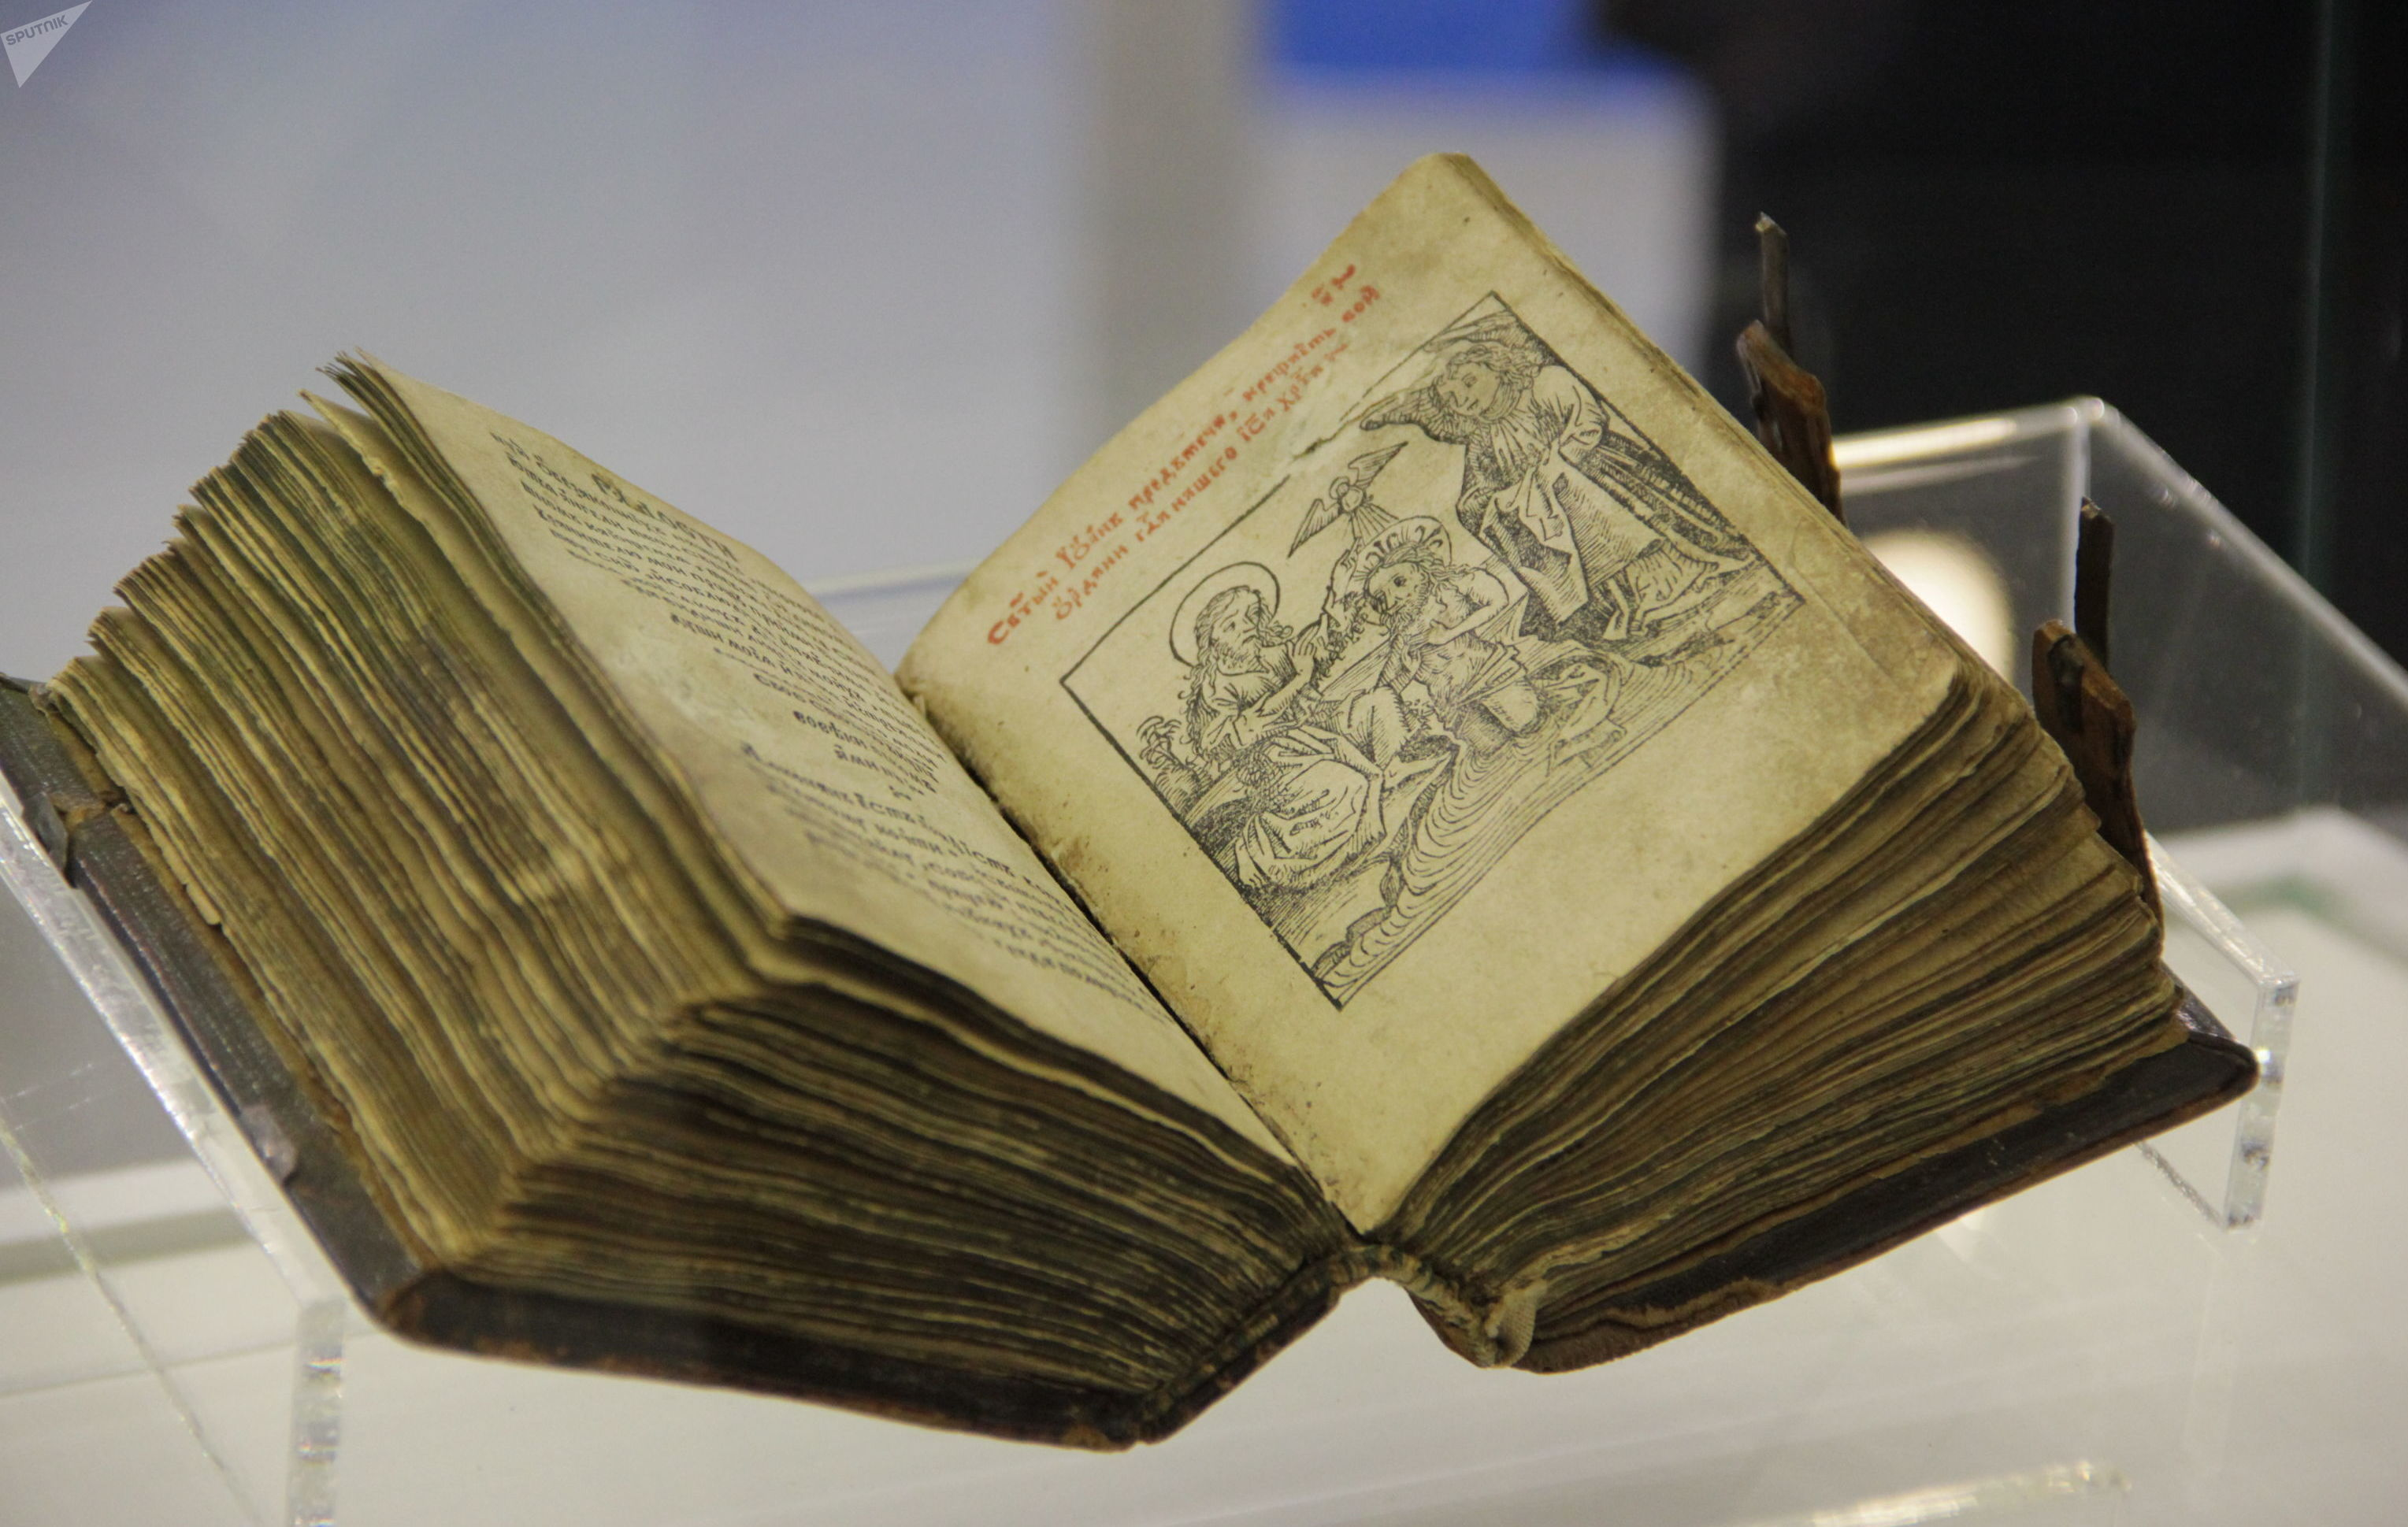
\includegraphics[width=0.5\textwidth]{susbook.jpg}
    \caption{Il (presto) famoso libro di Andrea.}
\end{figure}

Il libro è composto da $N$ pagine, numerate da $1$ a $N$. Le pagine possono essere mostrate in ordine
sparso (ossia è possibile ordinarle in un ordine diverso da $1,2\dots,N$).
Andrea vuole sapere se è possibile creare un ordinamento tale che, prese $3$ pagine consecutive
del libro, i numeri delle pagine sommati siano divisibili per $3$.

Ad esempio, se il libro avesse $6$ pagine, potrebbero essere ordinate nel seguente modo:
$$[3, 2, 1, 6, 5, 4]$$
In modo tale che la proprietà valga per tutte le triplette consecutive:
\begin{itemize}
    \item $3+2+1 = 3\cdot2$
    \item $2+1+6 = 3\cdot3$
    \item $1+6+5 = 3\cdot4$
    \item $6+5+4 = 3\cdot5$
\end{itemize}

Scrivi un ordinamento valido per le pagine del libro di Andrea!

\begin{warning}
    Possono esistere più soluzioni ottimali. In tal caso, qualsiasi delle soluzioni ottimali verrà considerata corretta.
\end{warning}

\Implementation

Dovrai sottoporre un unico file, con estensione \texttt{.cpp}.

\begin{warning}
    Tra gli allegati a questo task troverai un template \texttt{bookpages.cpp} con un esempio di implementazione.
\end{warning}

Il file di input è composto da $1$ riga:
\begin{itemize}
    \item Riga 1: l'intero $N$.
\end{itemize}

Il file di output è composto da $1$ riga:
\begin{itemize}
    \item Riga 1: la risposta al problema.
\end{itemize}

% % % % % % % % % % % % % % % % % % % % % % % % % % % % % % % % % % % % % % % % % % %
% % % % % % % % % % % % % % % % % % % % % % % % % % % % % % % % % % % % % % % % % % %

\Constraints

\begin{itemize}[nolistsep, itemsep=2mm]
    \item $3 \le N \le 1\:000\:000$.
    \item Si può dimostrare che esiste sempre un ordinamento valido.
\end{itemize}

% % % % % % % % % % % % % % % % % % % % % % % % % % % % % % % % % % % % % % % % % % %
% % % % % % % % % % % % % % % % % % % % % % % % % % % % % % % % % % % % % % % % % % %

\Scoring

Il tuo programma verrà testato su diversi test case raggruppati in subtask.
Per ottenere il punteggio relativo ad un subtask,
è necessario risolvere correttamente tutti i test che lo compongono.

\IIOTsubtask{0}{1}{Casi d'esempio.}

\IIOTsubtask{30}{1}{$N \le 8$}

\IIOTsubtask{50}{1}{$N \le 1\:000$}

\IIOTsubtask{20}{1}{Nessuna limitazione aggiuntiva.}


% % % % % % % % % % % % % % % % % % % % % % % % % % % % % % % % % % % % % % % % % % %
% % % % % % % % % % % % % % % % % % % % % % % % % % % % % % % % % % % % % % % % % % %

\Examples

\begin{example}
    \exmpfile{bookpages.input0.txt}{bookpages.output0.txt}%
    \exmpfile{bookpages.input1.txt}{bookpages.output1.txt}%
    \exmpfile{bookpages.input2.txt}{bookpages.output2.txt}%
\end{example}

% % % % % % % % % % % % % % % % % % % % % % % % % % % % % % % % % % % % % % % % % % %
% % % % % % % % % % % % % % % % % % % % % % % % % % % % % % % % % % % % % % % % % % %

\Explanation

Nei tre casi d'esempio, le permutazioni sono valide. Nota bene che non sono le uniche permutazioni valide,
ad esempio nel primo caso anche la permutazione \texttt{2 1 6 5 4 3} è valida.